\par Ce chapitre contient les diagrammes de classes représentant le logiciel codé. Les diagrammes de l'itération trois ont été complétés à partir du code pour ajouter les détails d'intégration dans le diagrammes (méthodes privées par exemple).

\section{Paquetage interpreteurlir.donnees(.litteraux)}
\begin{center}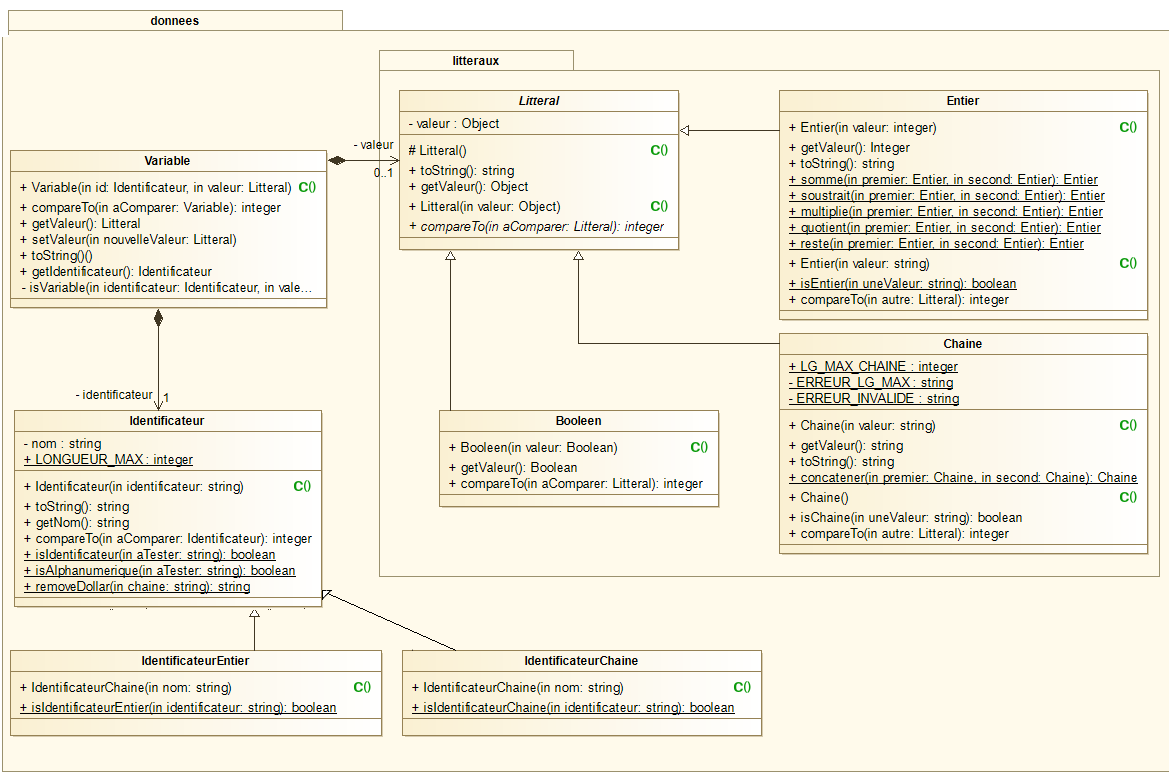
\includegraphics[scale=0.55]{fichiers/dossierPartieConception/img/COO/PackageDonnees}\end{center}

\section{Paquetage interpreteurlir.expressions}
\begin{center}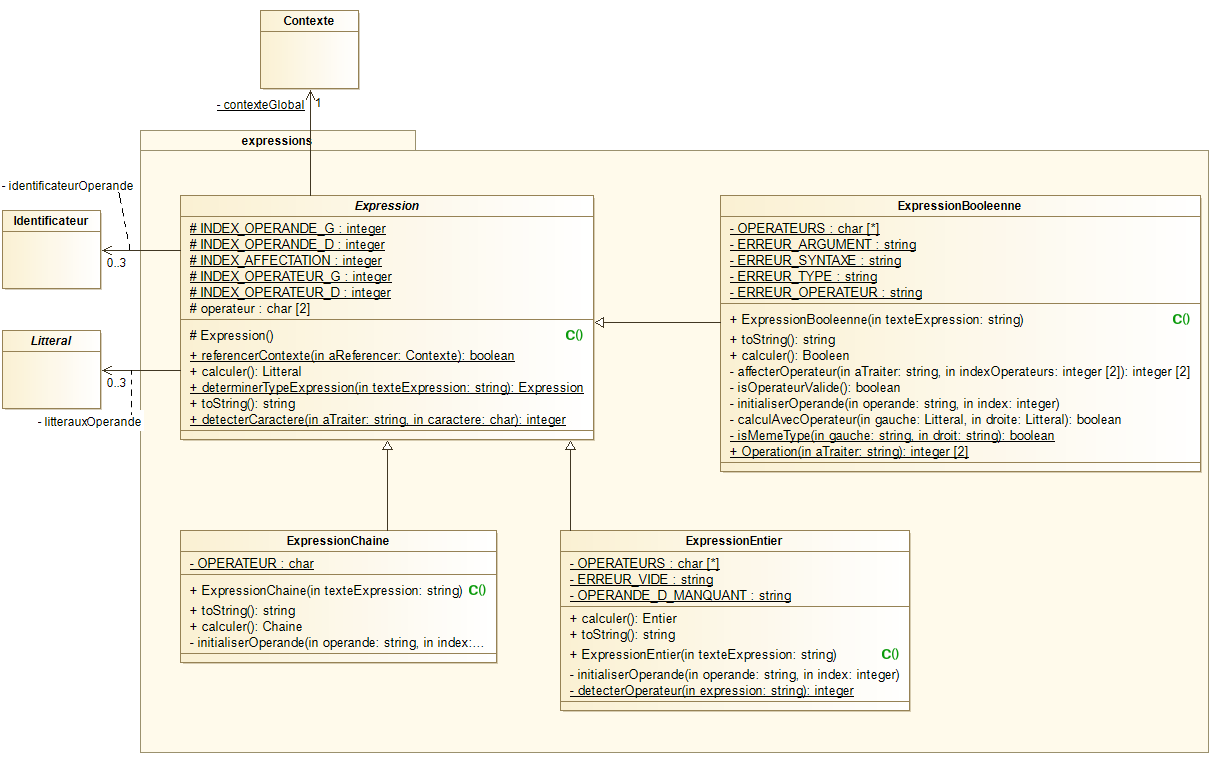
\includegraphics[scale=0.55]{fichiers/dossierPartieConception/img/COO/PackageExpression}\end{center}

\section{Paquetage interpreteurlir.programmes}
\begin{center}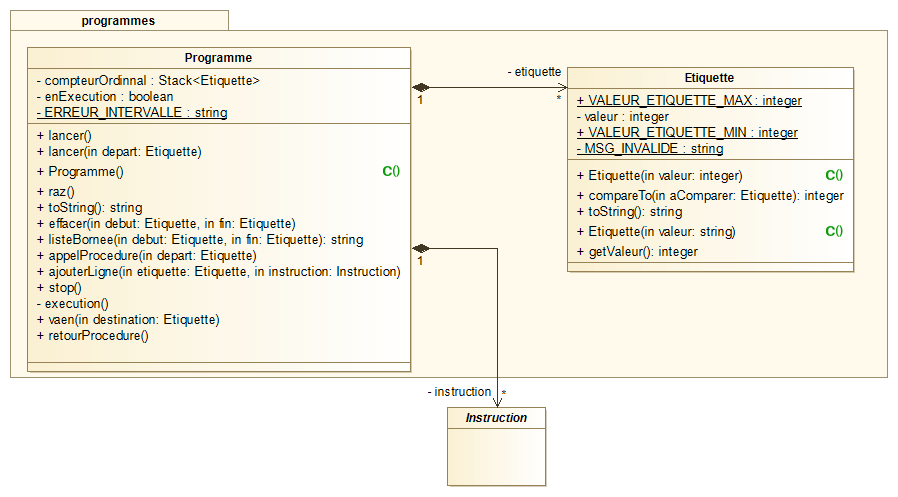
\includegraphics[scale=0.55]{fichiers/dossierPartieConception/img/COO/PackageProgrammes}\end{center}

\section{Paquetage interpreteurlir.motscles}
\begin{center}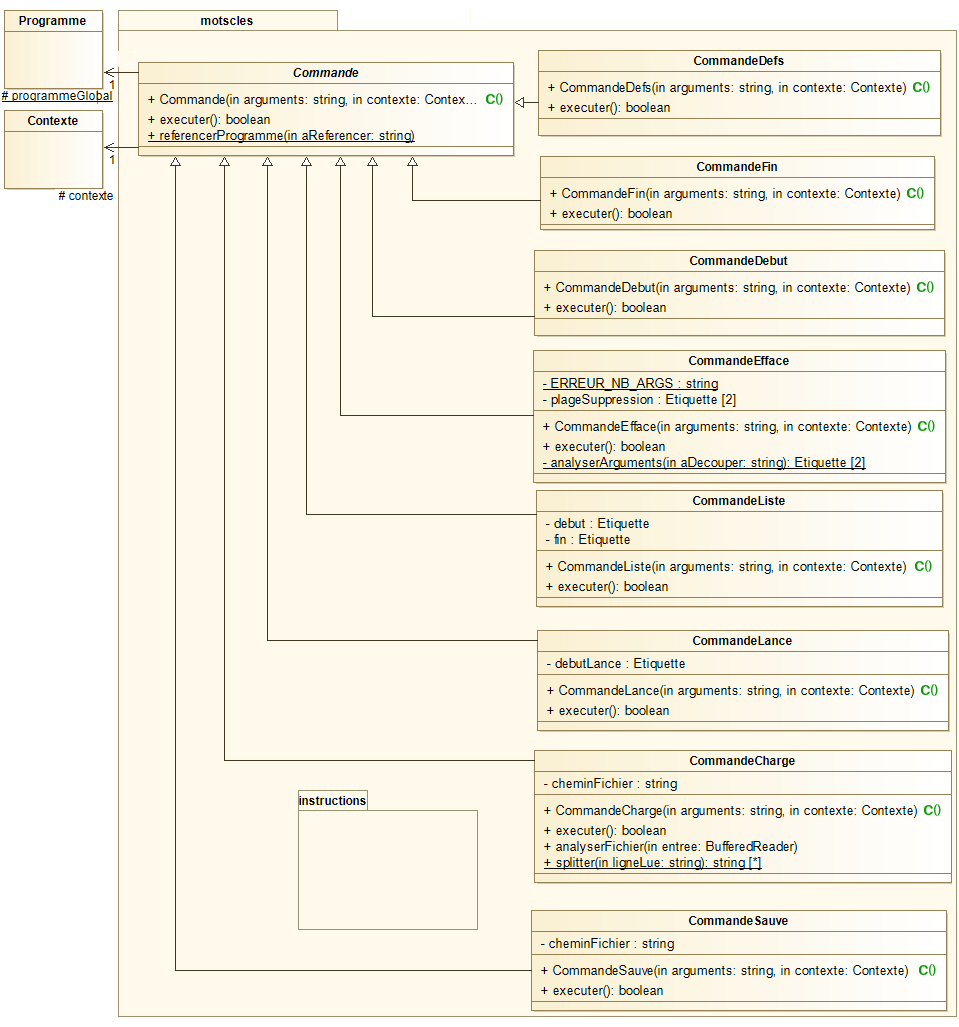
\includegraphics[scale=0.60]{fichiers/dossierPartieConception/img/COO/PackageMotscles}\end{center}

\section{Paquetage interpreteurlir.motscles.instructions}
\begin{center}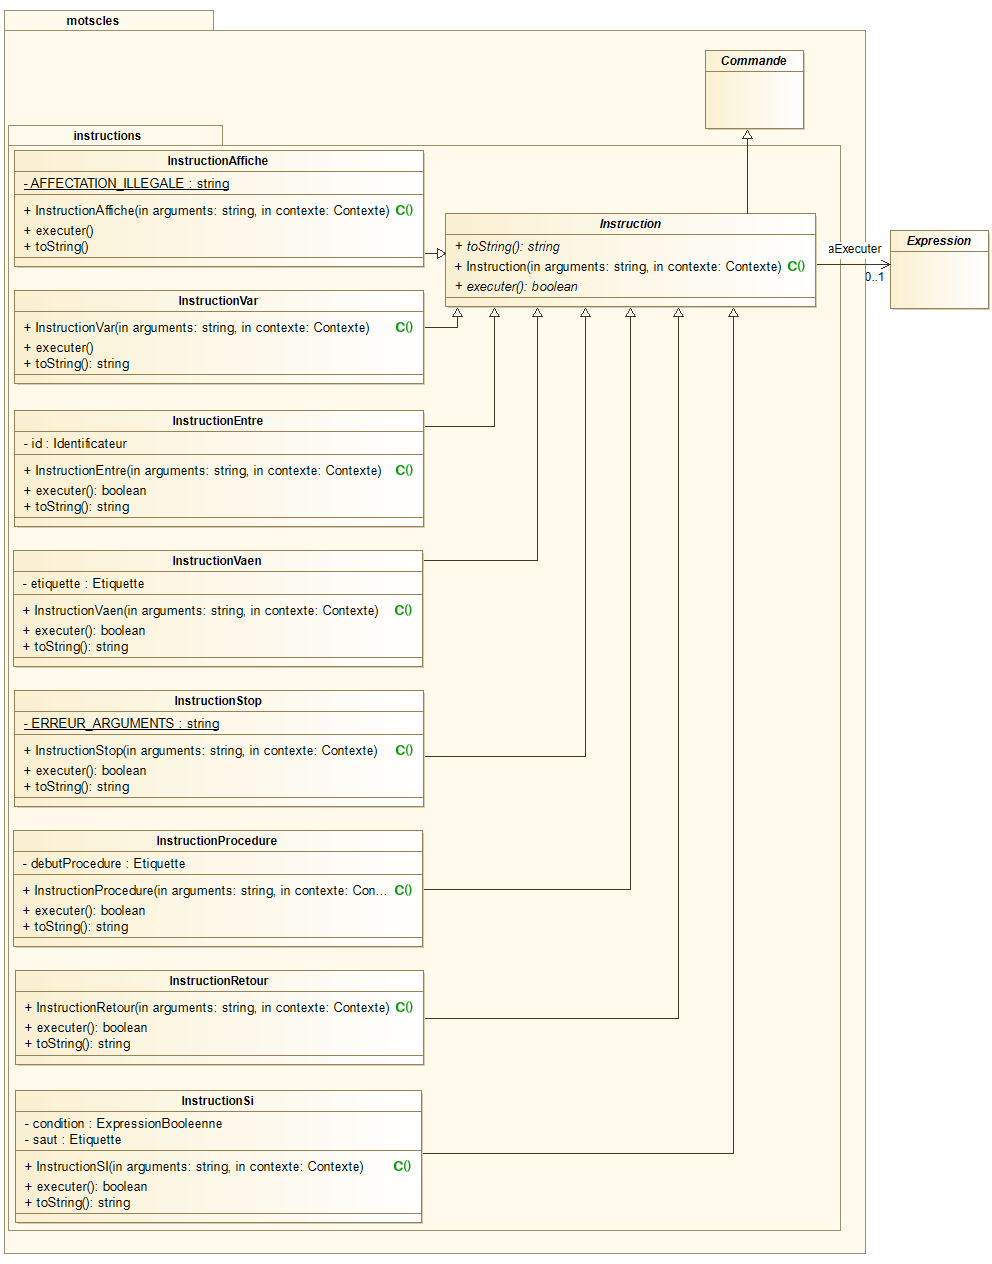
\includegraphics[scale=0.60]{fichiers/dossierPartieConception/img/COO/PackageInstruction}\end{center}

\section{Paquetage interpreteurlir}
\begin{center}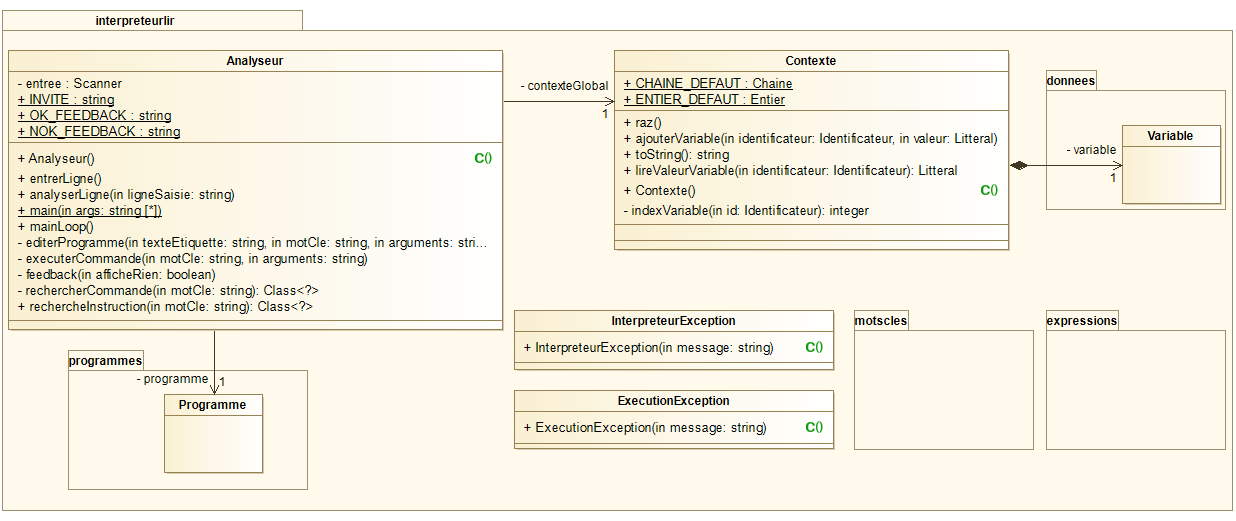
\includegraphics[scale=0.55]{fichiers/dossierPartieConception/img/COO/PackageInterpreteurlir}\end{center}